\documentclass[12pt]{article}

% Paquetes necesarios
\usepackage{float}
\usepackage{graphicx}
\usepackage[utf8]{inputenc}
\usepackage[T1]{fontenc}
\usepackage[spanish]{babel}
\usepackage{amsmath, amssymb}
\usepackage{listings}
\usepackage{color}
\usepackage{hyperref}
\usepackage{geometry}
\geometry{a4paper, margin=2.5cm}

% Configuración de listings para código C++ y Python
\definecolor{codegray}{rgb}{0.95,0.95,0.95}
\lstset{
  backgroundcolor=\color{codegray},
  basicstyle=\ttfamily\footnotesize,
  frame=single,
  breaklines=true,
  columns=fullflexible,
  showstringspaces=false
}

% Datos del documento
\title{Investigaciones Extras}
\author{Efraín Retana Segura \\ Curso: Estructuras Discretas}
\date{\today}

\begin{document}

\maketitle

\section*{Introducción}
Este documento recopila una serie de conceptos fundamentales relacionados con buenas prácticas y herramientas para el desarrollo en Python y C++, como los motores de prueba, la medición de tiempo, la refactorización y el perfilado del código. Estos temas surgen a partir de las sugerencias del profesor en las clases de \textbf{estructuras discretas}, con el objetivo de profundizar en herramientas que pueden ser útiles tanto en el presente como en el futuro profesional del estudiante. El contenido aquí expuesto busca ser comprensible y útil según el entendimiento del autor (estudiante).

\section{Testing Engine (Motor de Pruebas en Python y C++)}

\subsection*{¿Qué es un Testing Engine?}
Un \textbf{Testing Engine} es una herramienta o conjunto de herramientas que permiten automatizar la verificación del correcto funcionamiento de un programa. Su propósito es asegurar que las distintas partes del código, como funciones o clases, devuelvan los resultados esperados ante determinadas entradas.

\begin{figure}[H]
    \centering
    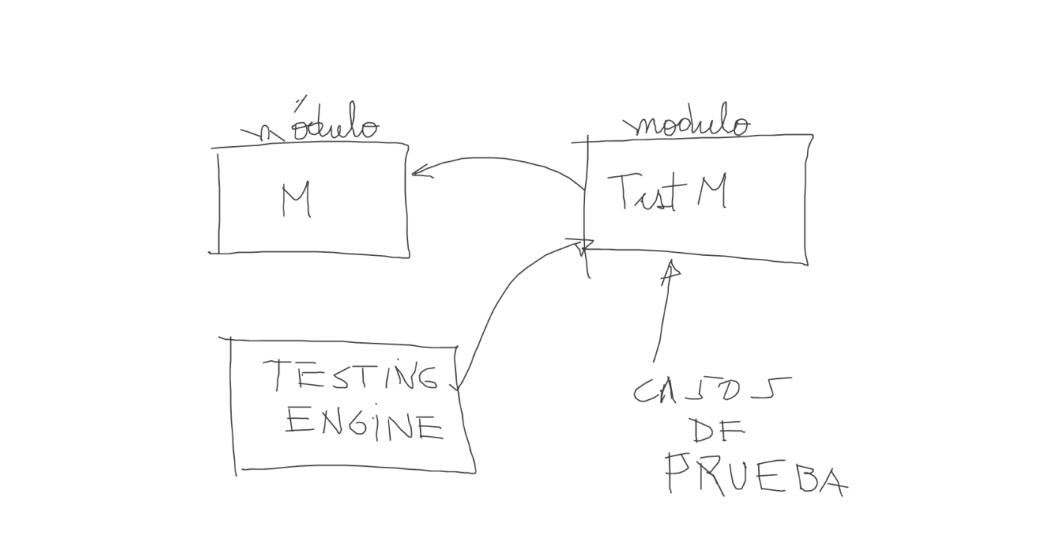
\includegraphics[width=0.5\linewidth]{Imagenes/Capture.PNG}
    \caption{Tomado de la clase de estructuras discretas del 3 de marzo de 2025.}
    \label{fig:testing-engine}
\end{figure}

\subsection*{Pruebas en Python y C++}
Para validar el comportamiento correcto del código, se utilizan motores de pruebas. Estas herrmamientas permiten automatizar la verificacíón de que las funciones y módulos del pograma se comporten como se espera. En el caso de \textbf{C++}, uno de los motores de prueba más populares es \textbf{Google Test}, desarrollado por Google.Permite realizar pruebas unitarias utilizando macros como \texttt{EXPECT\_EQ} para comparar resultados esperados con los reales, facilitando la detección de errores en etapas tempranas del desarrollo del programa. \\

En \textbf{Python}, existen varias opciones según el nivel de complejidad del proyecto:
\begin{itemize}
    \item \textbf{unittest}: Es el modulo oficial incluido en la biblioteca estándar de Python. Utiliza clases derivadas de \texttt{unittest.TestCase} y proporciona una estructura formal para organizar las pruebas.
    \item\textbf{pytest}: Es una herramienta externa muy popular por su sintaxis simple y poderosa. Permite escribir pruebas como funciones normales y cuenta con soporte para fixtures, parametrización y plugins. 
    \item\textbf{doctest}: Permite incrustar pruebas dentro de los mismos docstrings de las funciones. Es útil para documentación activa y para validar ejemplos sencillos.
\end{itemize}
\subsection*{Ejemplo con Google Test}
\begin{lstlisting}[language=C++]
#include <gtest/gtest.h>

int suma(int a, int b) {
    return a + b;
}

TEST(SumaTest, Positivos) {
    EXPECT_EQ(suma(2, 3), 5);
}
int main(int argc, char ** argv){
::testing::InitGoogleTest(&argc, argv);
    return RUN_ALL_TESTS();
}
\end{lstlisting}

Al compilar y ejecutar este código, se obtiene una salida parecida a la siguiente:
\begin{lstlisting}
    [==========] Running 1 test from 1 test case.
[----------] Global test environment set-up.
[----------] 1 test from SumaTest
[ RUN      ] SumaTest.Positivos
[       OK ] SumaTest.Positivos (0 ms)
[----------] 1 test from SumaTest (0 ms total)

[----------] Global test environment tear-down
[==========] 1 test from 1 test case ran. (0 ms total)
[  PASSED  ] 1 test.
\end{lstlisting}

\subsection*{Ejemplos en Python} 
\subsection*{1. unittest} 
\begin{lstlisting}[language=Python] 
import unittest

def suma(a, b):
    return a + b

class TestSuma(unittest.TestCase):
    def test_suma(self):
        self.assertEqual(suma(2, 3), 5)

if __name__ == '__main__':
    unittest.main()
\end{lstlisting}

Al ejecutar este script en la terminal, la salida será similiar a la siguiente:

\begin{lstlisting}
.
----------------------------------------------------------------------
Ran 1 test in 0.000s

OK
\end{lstlisting}

\subsection*{2. pytest}

\begin{lstlisting}[language=Python]
def suma(a, b):
    return a + b

def test_suma():
    assert suma(2, 3) == 5
\end{lstlisting}

Para ejecutar este test, se guarda el archivo (por ejemplo como \texttt{test\_suma.py}) y se ejecuta desde la terminal con:

\begin{lstlisting}
    pytest test_suma.py
\end{lstlisting}

La salida esperada sería algo como:

\begin{lstlisting}
============================= test session starts =============================
collected 1 item

test_suma.py .                                                        [100%]

============================== 1 passed in 0.01s ==============================
\end{lstlisting}

\subsection*{3. doctest}

\begin{lstlisting}[language=Python]
def suma(a, b):
    """
    >>> suma(2, 2)
    4
    >>> suma(-1, 1)
    0
    """
    return a + b

if __name__ == "__main__":
    import doctest
    doctest.testmod()
\end{lstlisting}
La ejecución normal del script (sin errores) no produce salida visible:

\begin{lstlisting}
#Sin salida si todo es correcto...
\end{lstlisting}

Sin embargo, si se ejecuta detallado (verbose mode), se obtiene una salida como esta:

\begin{lstlisting}
Trying:
    suma(2, 2)
Expecting:
    4
ok
Trying:
    suma(-1, 1)
Expecting:
    0
ok
1 items had no tests:
    __main__
1 items passed all tests:
   2 tests in __main__.suma
2 tests in 2 items.
2 passed and 0 failed.
Test passed.
\end{lstlisting}

\section{Medición de tiempo en Python y C++}

\subsection*{Python-timeit}
En python, la forma más precisa y común de medir el tiempo de ejecución de fragmentos de código es como el módulo \texttt{timeit}. Este módulo evita interferencias externas (como recoleccion de datos basura etc) y es ideal para microbenchmarks(Pruebas de rendimiento en partes especificas del código)

\begin{lstlisting} [language = Python]
import timeit

def suma(a, b):
    return a + b
#Medir cuanto tarda en ejecutarse suma(2, 3) 10000 veces
tiempo = timeit('suma(2,3)', setup='from __main__ import suma', number=100000)

print(f"Tiempo promedio: {tiempo:.6f} segundos")
\end{lstlisting}

\textbf{Salida esperada:}
\begin{lstlisting}
    Tiempo promedio: 0.012345 segundos
\end{lstlisting}

\subsection*{C++ - std::chrono}
En C++, se puede usar la libreria estándar \texttt{<chrono>} para medir el tiempo con alta precisión 

\begin{lstlisting} [language = C++]
#include <iostream>
#include <chrono>

int suma(int a, int b) {
    return a + b;
}

int main() {
    auto inicio = std::chrono::high_resolution_clock::now();

    for (int i = 0; i < 100000; ++i)
        suma(2, 3);

    auto fin = std::chrono::high_resolution_clock::now();
    std::chrono::duration<double> duracion = fin - inicio;

    std::cout << "Tiempo: " << duracion.count() << " segundos" << std::endl;
    return 0;
}
\end{lstlisting}

\textbf{Salida esperada de la consola:}

\begin{lstlisting}
    Tiempo: 0.003812 segundos
\end{lstlisting}

\subsection*{Datos a tomar sobre timeit y chrono}
Tanto para el modulo de Python y la libreria chrono, el tiempo de lo que queramos analizar dependera mucho de la maquina que utilicemos por esto no tomar a consideración lo que toma aqui, se pueden hacer pruebas en las maquinas del lector para poder comprobar empiricamente que los analisis de tiempo funcionan para los 2 lenguajes.

\section{Refactorización (Refactoring)}

\textbf{Refactoring} o refactorización en español es el proceso de modificar la estructura interna del código sin cambiar su comportamiento externo. El objetivo es mejorar la legibilidad, mantenibilidad y eficiencia del código.

\subsection*{Ejemplo de refactorización en Python}

\textbf{Antes:}
\begin{lstlisting}[language=Python]
def operacion(a, b, tipo):
    if tipo == "suma":
        return a + b
    elif tipo == "resta":
        return a - b
\end{lstlisting}

\textbf{Después (refactorizado):}
\begin{lstlisting}[language=Python]
def sumar(a, b):
    return a + b

def restar(a, b):
    return a - b
\end{lstlisting}

Esta mejora separa responsabilidades y hace que el código sea más modular, facilitando pruebas y mantenimiento.
\section{Profiling (Perfilado de Rendimiento)}
El perfilado permite analizar qué partes del código consumen más recursos, ayudando a identificar cuellos de botella en el rendimiento.

\subsection{Profiling en Python con \texttt{cProfile}}

\begin{lstlisting}[language = Python]
import cProfile
def suma():
    total = 0
    for i in range(1000):
        total += i
    return total

cProfile.run('suma()')
\end{lstlisting}

\textbf{Salida:}
\begin{lstlisting}
         4 function calls in 0.000 seconds

   Ordered by: standard name

   ncalls  tottime  percall  cumtime  percall filename:lineno(function)
        1    0.000    0.000    0.000    0.000 test.py:3(suma)
        1    0.000    0.000    0.000    0.000 {built-in method builtins.exec}
        1    0.000    0.000    0.000    0.000 {method builtins.print}
\end{lstlisting}

\subsection*{Profiling en C++ con herramientas externas}

En C++, el profiling suele hacerse con herramientas externas como:

\begin{itemize}
    \item \textbf{gprof}: Herramienta de GNU que permite analizar la ejecución del programa y visualizar qué funciones consumen más tiempo.
    \item \textbf{Valgrind + Callgrind}: Detecta fugas de memoria y puede analizar el tiempo relativo de ejecución de funciones.
    \item \textbf{perf (Linux)}: Utilidad poderosa de análisis de rendimiento de bajo nivel.
\end{itemize}

Un uso básico de \texttt{gprof} sería compilar así:

\begin{lstlisting}
g++ -pg programa.cpp -o programa
./programa
gprof programa gmon.out > reporte.txt
\end{lstlisting}

\newpage
\begin{thebibliography}{9}

\bibitem{python-timeit}
Python Software Foundation. (n.d.). \textit{timeit — Measure execution time of small code snippets}. Python 3.12. Recuperado de \url{https://docs.python.org/3/library/timeit.html}

\bibitem{python-unittest}
Python Software Foundation. (n.d.). \textit{unittest — Unit testing framework}. Python 3.12. Recuperado de \url{https://docs.python.org/3/library/unittest.html}

\bibitem{python-cprofile}
Python Software Foundation. (n.d.). \textit{cProfile — Profile deterministic profiling of Python programs}. Python 3.12. Recuperado de \url{https://docs.python.org/3/library/cprofile.html}

\bibitem{googletest}
Google. (n.d.). \textit{GoogleTest: Google Testing and Mocking Framework}. Recuperado de \url{https://github.com/google/googletest}

\bibitem{cpp-chrono}
ISO C++. (n.d.). \textit{<chrono> - cppreference.com}. Recuperado de \url{https://en.cppreference.com/w/cpp/chrono}

\bibitem{fowler}
Fowler, M. (2018). \textit{Refactoring: Improving the design of existing code} (2nd ed.). Addison-Wesley Professional.

\bibitem{google-software}
Sadowski, C., \& Zimmermann, T. (Eds.). (2019). \textit{Software engineering at Google: Lessons learned from programming over time}. O'Reilly Media.

\bibitem{chatgpt}
OpenAI. (2025). \textit{Asistencia personalizada proporcionada por ChatGPT para investigación estudiantil sobre herramientas de programación}. Recuperado de \url{https://chat.openai.com/}

\end{thebibliography}

\end{document}